% Options for packages loaded elsewhere
\PassOptionsToPackage{unicode}{hyperref}
\PassOptionsToPackage{hyphens}{url}
%
\documentclass[
]{article}
\usepackage{amsmath,amssymb}
\usepackage{lmodern}
\usepackage{ifxetex,ifluatex}
\ifnum 0\ifxetex 1\fi\ifluatex 1\fi=0 % if pdftex
  \usepackage[T1]{fontenc}
  \usepackage[utf8]{inputenc}
  \usepackage{textcomp} % provide euro and other symbols
\else % if luatex or xetex
  \usepackage{unicode-math}
  \defaultfontfeatures{Scale=MatchLowercase}
  \defaultfontfeatures[\rmfamily]{Ligatures=TeX,Scale=1}
\fi
% Use upquote if available, for straight quotes in verbatim environments
\IfFileExists{upquote.sty}{\usepackage{upquote}}{}
\IfFileExists{microtype.sty}{% use microtype if available
  \usepackage[]{microtype}
  \UseMicrotypeSet[protrusion]{basicmath} % disable protrusion for tt fonts
}{}
\makeatletter
\@ifundefined{KOMAClassName}{% if non-KOMA class
  \IfFileExists{parskip.sty}{%
    \usepackage{parskip}
  }{% else
    \setlength{\parindent}{0pt}
    \setlength{\parskip}{6pt plus 2pt minus 1pt}}
}{% if KOMA class
  \KOMAoptions{parskip=half}}
\makeatother
\usepackage{xcolor}
\IfFileExists{xurl.sty}{\usepackage{xurl}}{} % add URL line breaks if available
\IfFileExists{bookmark.sty}{\usepackage{bookmark}}{\usepackage{hyperref}}
\hypersetup{
  pdftitle={Species ID Guide Template},
  pdfauthor={Payton Arthur},
  hidelinks,
  pdfcreator={LaTeX via pandoc}}
\urlstyle{same} % disable monospaced font for URLs
\usepackage[margin=1in]{geometry}
\usepackage{longtable,booktabs,array}
\usepackage{calc} % for calculating minipage widths
% Correct order of tables after \paragraph or \subparagraph
\usepackage{etoolbox}
\makeatletter
\patchcmd\longtable{\par}{\if@noskipsec\mbox{}\fi\par}{}{}
\makeatother
% Allow footnotes in longtable head/foot
\IfFileExists{footnotehyper.sty}{\usepackage{footnotehyper}}{\usepackage{footnote}}
\makesavenoteenv{longtable}
\usepackage{graphicx}
\makeatletter
\def\maxwidth{\ifdim\Gin@nat@width>\linewidth\linewidth\else\Gin@nat@width\fi}
\def\maxheight{\ifdim\Gin@nat@height>\textheight\textheight\else\Gin@nat@height\fi}
\makeatother
% Scale images if necessary, so that they will not overflow the page
% margins by default, and it is still possible to overwrite the defaults
% using explicit options in \includegraphics[width, height, ...]{}
\setkeys{Gin}{width=\maxwidth,height=\maxheight,keepaspectratio}
% Set default figure placement to htbp
\makeatletter
\def\fps@figure{htbp}
\makeatother
\setlength{\emergencystretch}{3em} % prevent overfull lines
\providecommand{\tightlist}{%
  \setlength{\itemsep}{0pt}\setlength{\parskip}{0pt}}
\setcounter{secnumdepth}{-\maxdimen} % remove section numbering
\usepackage[font=small,format=plain,labelfont=bf,up,textfont=normal,up,justification=justified,singlelinecheck=false]{caption}
\ifluatex
  \usepackage{selnolig}  % disable illegal ligatures
\fi

\title{Species ID Guide Template}
\author{Payton Arthur}
\date{10/18/2021}

\begin{document}
\maketitle

\newpage

\hypertarget{pagurus-hirsutiusculus-hairy-hermit-crab}{%
\section{\texorpdfstring{\emph{Pagurus hirsutiusculus} (Hairy Hermit
Crab)}{Pagurus hirsutiusculus (Hairy Hermit Crab)}}\label{pagurus-hirsutiusculus-hairy-hermit-crab}}

\hypertarget{description}{%
\subsection{Description}\label{description}}

Each organism can be black, brown or dark green (Meschkat et al., 2014).
Shell shape can vary but shape of the actual body is fairly consistent
with the shield of the carapace (most cranial part of the back of the
crab) being less long than it is wide (Jensen, 2014). Body size can
reach 2 cm (Meschkat et al., 2014). The hairy hermit crab has hairs
along its body (Meschkat et al., 2014). However, the amount of hairs can
vary from one individual to another (Jensen, 2014). On its walking legs,
these crabs have a white band by the last joint (Meschkat et al., 2014).
More white bands may be present if the individual is young (Jensen,
2014). Also, their walking legs often have at most two blue dots on each
leg though these may be more difficult to see (Meschkat et al., 2014).
Small light rings encircle their antennae (Meschkat et al., 2014).

\textbf{Species lookalike}\\
It possesses one lookalike species: Pagurus carinus (the greenmark
hermit crab) (Meschkat et al., 2014). However, this crab lacks rings on
the antennae, possesses spiny claws and has a carapace that only reaches
1 cm which is half the size as hairy hermit crabs (Harbo, 2011).

\textbf{Range, Habitat, Diet, Foraging Mode and Reproduction}\\
These crabs can be found between California (Monterey) and Alaska
(Pribilof Islands) (Harbo, 2011). They live in protected areas including
the intertidal zone in tidepools protected by algae (Meschkat et al.,
2014; Harbo, 2011). Or, on the rare occasion, they may be found up to
110m subtidally (Harbo, 2011). These crabs are detrivores, thus they eat
dead organisms but will eat other live animals if available (Cowles,
2005b). They actively search for food by walking around (Jensen, 2014).
They undergo sexual reproduction and are oviparous meaning they lay eggs
(Kornienko, 2020).

\hypertarget{questions}{%
\subsection{Questions}\label{questions}}

\begin{enumerate}
\def\labelenumi{\arabic{enumi}.}
\tightlist
\item
  Are there hairs on the body?
\item
  Are there white bands around the last joints of the first two legs?
\item
  Are there rings circling around the antennae?
\end{enumerate}

\newpage

\hypertarget{figures}{%
\subsection{Figures}\label{figures}}

\begin{figure}

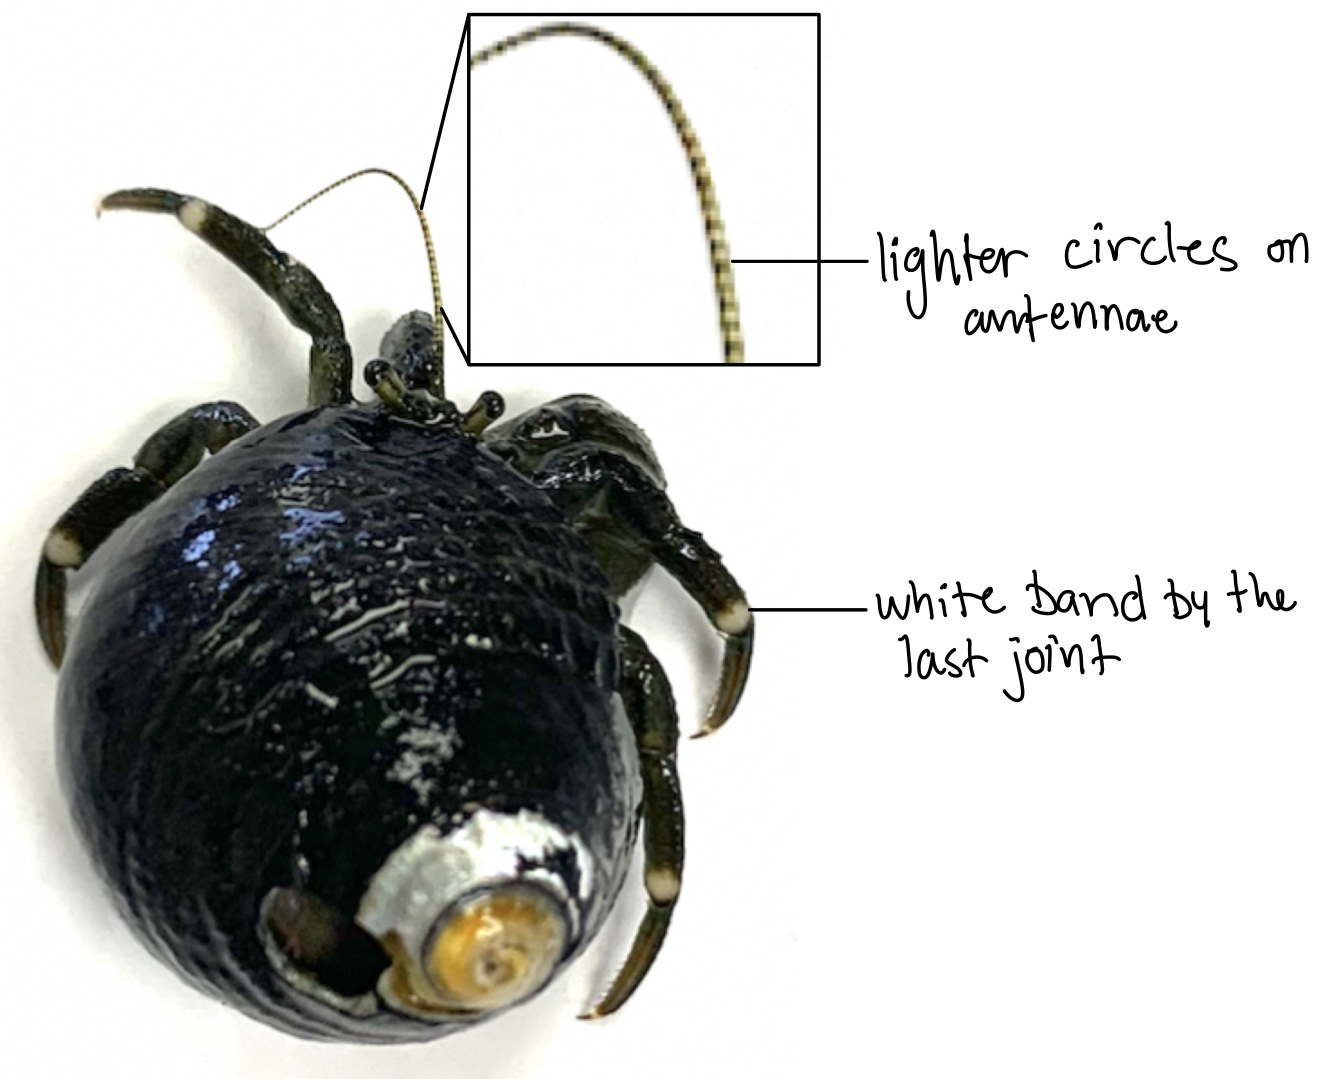
\includegraphics[width=0.5\linewidth,height=0.3\textheight]{/Users/P/Github/species-id-guide-p1234/images/hairy-hermit-full-labeled} \hfill{}

\caption{Figure 1. Photo of *Pagurus hirsutiusculus* including labeled diagnostic features}\label{fig:southern-right-whale}
\end{figure}

\begin{figure}

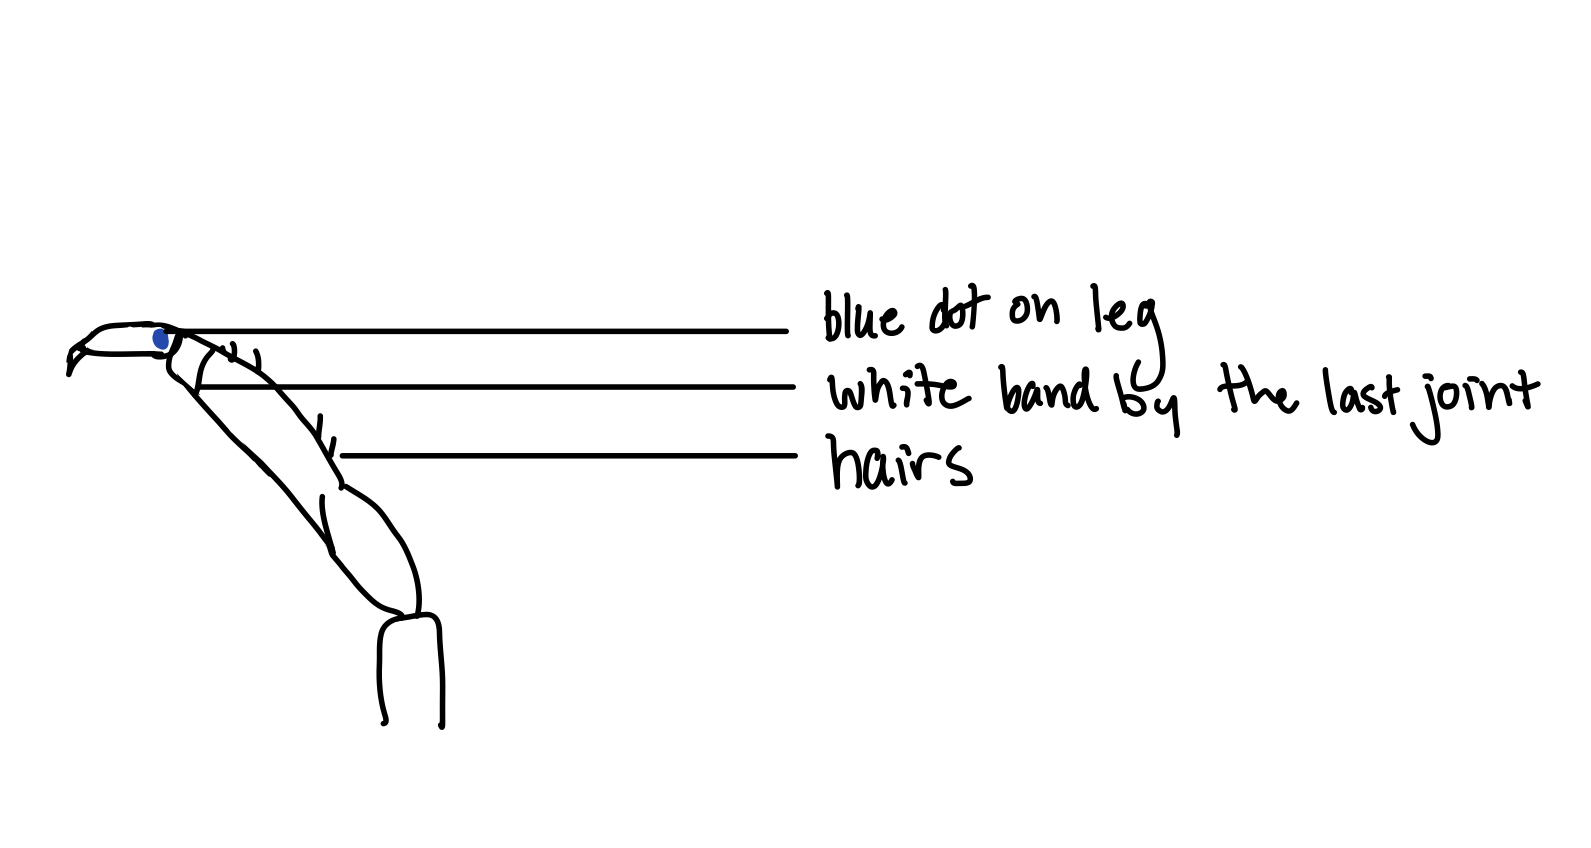
\includegraphics[width=0.5\linewidth,height=0.3\textheight]{/Users/P/Github/species-id-guide-p1234/images/hairy-hermit-leg-drawing} \hfill{}

\caption{Figure 2. Drawing of the leg of *Pagurus hirsutiusculus* including labeled diagnostic features}\label{fig:southern-right-whale-skull}
\end{figure}

\begin{figure}

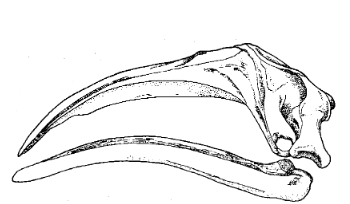
\includegraphics[width=0.5\linewidth,height=0.3\textheight]{/Users/P/Github/species-id-guide-p1234/images/southern-right-skull-lateral} \hfill{}

\caption{This is the skull of the southern right whale skull (lateral view), figure is left-aligned.}\label{fig:southern-right-whale-skull-lateral}
\end{figure}

\newpage

\hypertarget{balaena-mysticetus-bowhead-whale}{%
\section{\texorpdfstring{\emph{Balaena mysticetus} (Bowhead
whale)}{Balaena mysticetus (Bowhead whale)}}\label{balaena-mysticetus-bowhead-whale}}

\hypertarget{description-1}{%
\subsection{Description}\label{description-1}}

Bowhead whales are very rotund, but often have a distinct ``neck''
region. The head is large\ldots{} Text text text text. \textbf{Bold text
bold text bold text.} \emph{Italicized text italicized text italicized
text}. Text text text text. \textbf{Bold text bold text bold text.}
\emph{Italicized text italicized text italicized text}. Text text text
text. \textbf{Bold text bold text bold text.} \emph{Italicized text
italicized text italicized text}. Text text text text. \textbf{Bold text
bold text bold text.} \emph{Italicized text italicized text italicized
text}. Text text text text. \textbf{Bold text bold text bold text.}
\emph{Italicized text italicized text italicized text}. Text text text
text. \textbf{Bold text bold text bold text.} \emph{Italicized text
italicized text italicized text}. Text text text text. \textbf{Bold text
bold text bold text.} \emph{Italicized text italicized text italicized
text}. Text text text text. \textbf{Bold text bold text bold text.}
\emph{Italicized text italicized text italicized text}. Text text text
text. \textbf{Bold text bold text bold text.} \emph{Italicized text
italicized text italicized text}. Text text text text. \textbf{Bold text
bold text bold text.} \emph{Italicized text italicized text italicized
text}. Text text text text. \textbf{Bold text bold text bold text.}
\emph{Italicized text italicized text italicized text}. Text text text
text. \textbf{Bold text bold text bold text.} \emph{Italicized text
italicized text italicized text}.

\newpage

\hypertarget{figures-1}{%
\subsection{Figures}\label{figures-1}}

\begin{figure}
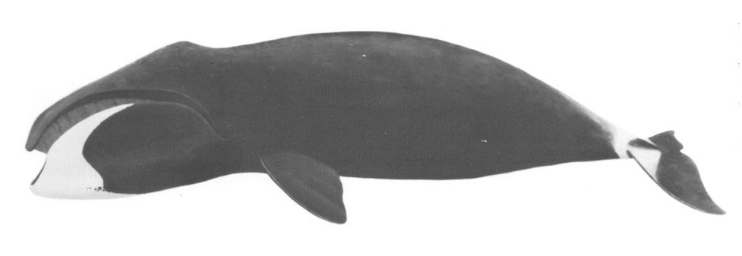
\includegraphics[width=0.5\linewidth,height=0.3\textheight]{/Users/P/Github/species-id-guide-p1234/images/bowhead} \caption{This is the bowhead whale, figure is centered.}\label{fig:bowhead-whale}
\end{figure}

\begin{figure}
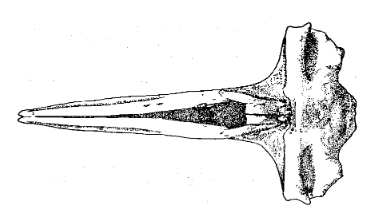
\includegraphics[width=0.5\linewidth,height=0.3\textheight]{/Users/P/Github/species-id-guide-p1234/images/bowhead-skull} \caption{This is the skull of the bowhead whale skull, figure is centered.}\label{fig:bowhead-whale-skull}
\end{figure}

\begin{figure}
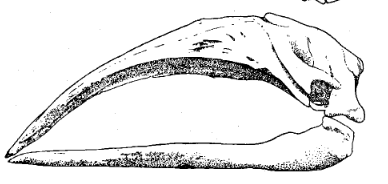
\includegraphics[width=0.5\linewidth,height=0.3\textheight]{/Users/P/Github/species-id-guide-p1234/images/bowhead-skull-lateral} \caption{This is the skull of the bowhead whale skull, figure is centered.}\label{fig:bowhead-whale-skull-lateral}
\end{figure}

\newpage

\hypertarget{questions-1}{%
\subsection{Questions}\label{questions-1}}

\begin{enumerate}
\def\labelenumi{\arabic{enumi}.}
\tightlist
\item
  Very interesting and useful question
\item
  Another wildly helpful question
\item
  A third, MOST fascinating question
\end{enumerate}

\newpage

\hypertarget{references}{%
\subsection{References}\label{references}}

\hypertarget{supplemental-information}{%
\section{Supplemental Information}\label{supplemental-information}}

\begin{longtable}[]{@{}llllll@{}}
\caption{Table 1. Whale morphometrics and other
infomration.}\tabularnewline
\toprule
Species & Length & Weight & Trophic Role & Diet & Reproduction \\
\midrule
\endfirsthead
\toprule
Species & Length & Weight & Trophic Role & Diet & Reproduction \\
\midrule
\endhead
Bowhead whale & 18..7-20.8 & 81542.79 - 90700 & predators & kril &
sexual \\
Southern right whale & 14.5-18.2 & 63576.92 - 79800 & predators & krill
& sexual \\
\bottomrule
\end{longtable}

\hypertarget{supplemental-information-1}{%
\section{Supplemental Information}\label{supplemental-information-1}}

\begin{longtable}[]{@{}lrr@{}}
\caption{Table 1. Hermit crab morphometrics and other
information.}\tabularnewline
\toprule
Individual & Shell Length (mm) & Claw Size (mm) \\
\midrule
\endfirsthead
\toprule
Individual & Shell Length (mm) & Claw Size (mm) \\
\midrule
\endhead
Hairy Hermit Crab 1 & 7 & 2.5 \\
Hairy Hermit Crab 2 & 18 & 6.5 \\
Grainyhand Crab 1 & 19 & 4.0 \\
Grainyhand Crab 2 & 32 & 7.0 \\
\bottomrule
\end{longtable}

\hypertarget{figures-2}{%
\subsection{Figures}\label{figures-2}}

\begin{figure}
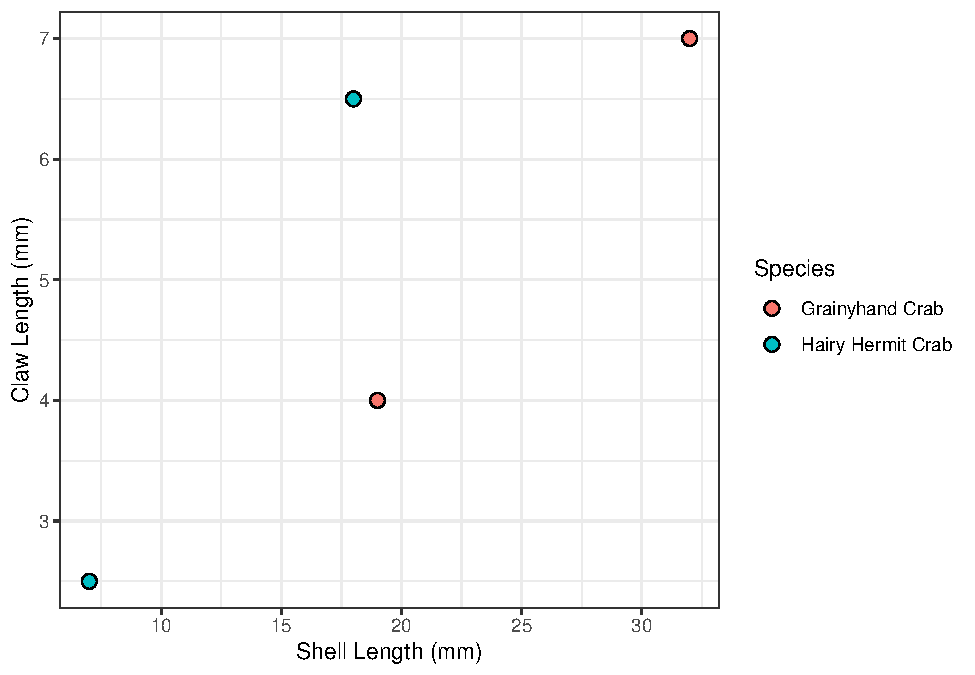
\includegraphics[width=0.5\linewidth,height=0.5\textheight]{species-id-crabs_files/figure-latex/unnamed-chunk-3-1} \caption{Supplementary Figure 1. Shell lenght and claw length compared by species in hermit crabs.}\label{fig:unnamed-chunk-3}
\end{figure}

\begin{figure}
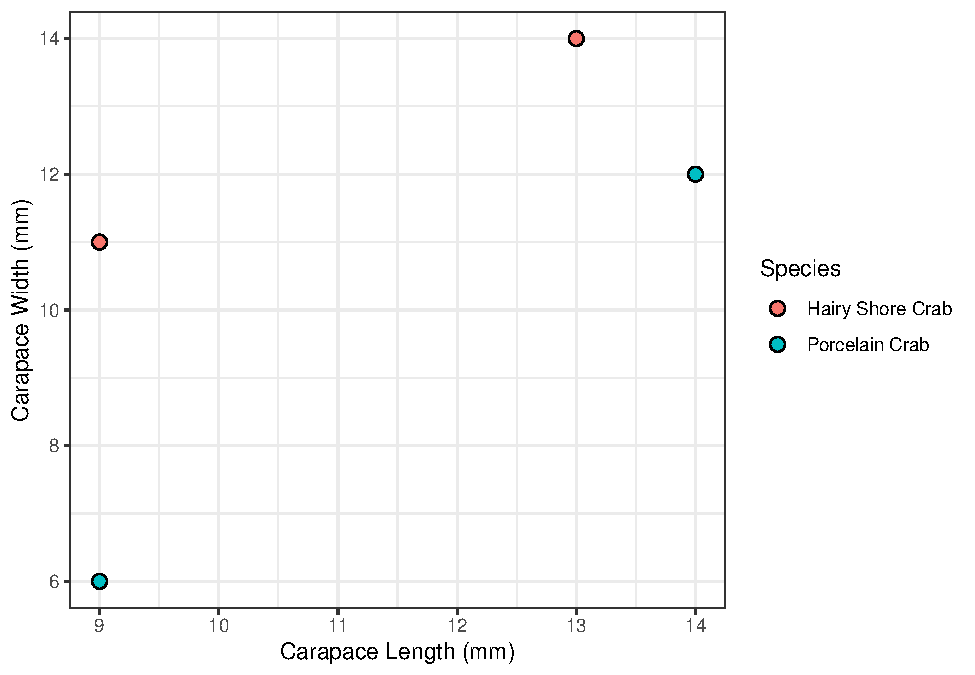
\includegraphics[width=0.5\linewidth,height=0.5\textheight]{species-id-crabs_files/figure-latex/unnamed-chunk-4-1} \caption{Supplementary Figure 2. Carapace lenght and width compared by species of shore crabs.}\label{fig:unnamed-chunk-4}
\end{figure}

\begin{figure}
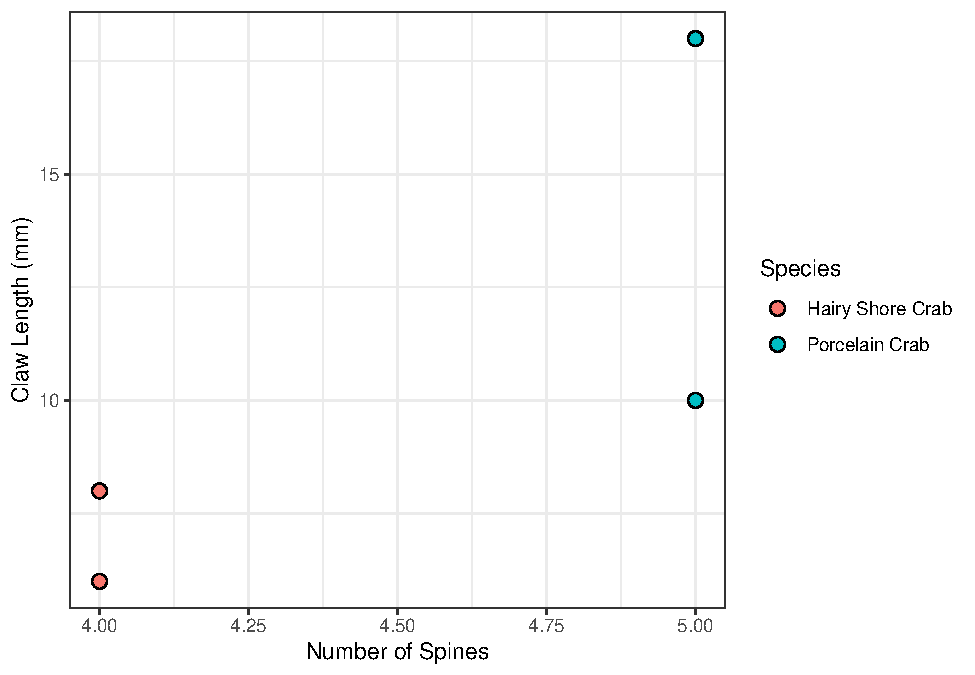
\includegraphics[width=0.5\linewidth,height=0.5\textheight]{species-id-crabs_files/figure-latex/unnamed-chunk-5-1} \caption{Supplementary Figure 3. Number of spines and claw length compared by species of shore crabs.}\label{fig:unnamed-chunk-5}
\end{figure}

\end{document}
